\documentclass[UTF8]{ctexart}
\usepackage{graphicx}
\usepackage{float}
\usepackage{geometry}
\usepackage{fancyhdr}
\usepackage{lastpage}
\usepackage{amsmath}
\usepackage{multicol}
\usepackage{multirow}
\usepackage{subfigure}
\geometry{left=2.54cm,right=2.54cm,top=3.18cm,bottom=3.18cm}%页边距
\pagestyle{fancy}
\lhead{
\includegraphics[scale=1]{sjtu-logo-red.pdf}}  
\rhead{生物医学工程领域开源软件综述} 
\cfoot{第 \thepage\ 页\ 共 \pageref{LastPage} 页} 

\newcommand{\enabstractname}{Abstract}

\begin{document}
\bibliographystyle{plain}
\begin{titlepage}
    \begin{center}
        
\includegraphics[width=0.8\textwidth]{sjtu-name-blue.pdf}\\[1cm]
        \textsc{\Huge \bfseries 课程报告}\\[1.5cm]
        
\includegraphics[width=0.3\textwidth]{sjtu-badge-blue.pdf}\\[0.5cm]    

        \Huge \bfseries{生物医学工程领域开源软件综述}\\[1cm]
        \Large \bfseries{518021910971 裴奕博}
    \end{center}
\end{titlepage}
\tableofcontents
\newpage

\begin{abstract}
    如今,开源软件已经成为了软件开发和共享的一大趋势。本文介绍了开源的概念,常用的几种开源协议,开源代码托管平台。列举了几个常用的生物医学工程领域的开源软件,并对开源的这一现象及其价值进行了讨论。
    
    \textbf{关键字:} 开源、开源协议、生物医学工程
\end{abstract}
%正文

\section{开源的概念}
开源(Open Source),是一种软件设计开发和分发的模式。在传统的软件发行模式中,开发者会以开放应用接口,编译为动态库等方式,对用户影藏源代码。而开源软件则不同,开源软件的源代码对所有开发者、用户和其他感兴趣的人员开放,在近年来的软件设计和分发中越来越受到开发者的欢迎。开源并不仅仅意味着可以开放访问的源代码,根据Open Source Init拟定的标准,此处将开源软件的理念和特点总结为如下几点\cite{opensourceinit}:
\begin{enumerate}
    \item 免费分发(Free Redistribution)。开源许可不应限制任何一方将软件作为包含来自多个不同来源的程序的聚合软件分发的组件进行销售或赠送。许可证不要求为此类销售支付特许权使用费或其他费用。
    \item 开放源代码(Source Code)。该程序必须包含源代码,并且必须允许以源代码和编译形式分发。如果某种形式的产品不附带源代码,则必须有一种广为人知的方式以不超过合理的复制成本获得源代码,最好是通过互联网免费下载。源代码必须是程序员修改程序的首选形式。不允许故意混淆源代码。不允许使用中间形式,例如预处理器或翻译器的输出。
    \item 允许衍生产品(Derived Work)。许可必须允许修改和衍生作品,并且必须允许它们按照与原始软件许可相同的条款进行分发。
    \item 作者源代码的完整性(Integrity of The Author's Source Code)。仅当许可证允许分发带有源代码的“补丁文件”以在构建时修改程序时,许可证才可以限制源代码以修改的形式分发。许可证必须明确允许分发从修改过的源代码构建的软件。许可证可能要求派生作品带有与原始软件不同的名称或版本号。
    \item 不得歧视任何开发者和组织(No Discrimination Against Persons or Groups)。许可证不得歧视任何个人或群体。
    \item 不得歧视任何应用领域(No Discrimination Against Fields of Endeavor)。许可证不得限制任何人在特定领域使用该程序。例如,它可能不会限制该程序用于企业或用于基因研究。
    \item 许可证的分发(Distribution of License)。程序附带的权利必须适用于得到分发程序的所有人,而无需这些方执行额外的许可。
    \item 独立于产品的许可(License Must Not Be Specific to a Product)。程序附带的权利不得取决于程序是否属于特定软件分发的一部分。如果该程序是从该分发中提取并在该程序的许可条款内使用或分发的,则该程序被重新分发的所有各方都应拥有与原始软件分发一起授予的权利相同的权利。
    \item 许可不得限制其他软件(License Must Not Restrict Other Software)。许可证不得对与许可软件一起分发的其他软件设置限制。例如,许可证不得坚持基于该软件开发的软件中的所有其他程序必须是开源软件。
    \item 许可必须是技术中立的(License Must Be Technology-Neutral)。许可的提供不得以任何单独的技术或界面风格为前提。
\end{enumerate}

\section{开源协议介绍}
开源协议指的是以上满足开源定义的协议,它们的共同特点是允许软件的免费使用、修改和共享。而根据所需开放程度的不同,提供了不同的开源协议,目前开源协议共有上百种之多。而其中常用的开源协议包括:GPL、LGPL、BSD、MIT、Mozilla和Apache。此处列举如下:\cite{opensourceinit}\cite{runoob}\cite{zhihuOpenSource}
\subsection{GPL协议}
GPL协议(GNU General Public License),全称GNU通用公共许可协议。GPL的开源程度在各种协议中最大。GPL的出发点是代码的开源/免费使用和引用/修改/衍生代码的开源/免费使用。GPL协议要求只要软件中包含了遵循 GPL 协议的产品或代码,该软件就必须也遵循 GPL许可协议,也就是必须开源免费,开放所有源代码,因此这个协议并不适合商用软件。

遵循GPL协议的开源软件数量很多,包括我们如今看到的Linux的各种发行版、gcc编译器等均采用了GPL协议。
\subsection{LGPL协议}
LGPL协议(GNU Lesser General Public License),全称GNU宽通用公共许可证,同样由GNU发行并推出,是GPL协议的一个衍生版本。由于GPL协议对商业软件不友好,GNU推出了允许商业软件通过类库引用(link)的方式使用 LGPL 类库,而不需要开源商业软件的代码的LGPL协议。这使得采用 LGPL 协议的开源代码可以被商业软件作为类库引用并发布和销售。

但是如果修改 LGPL 协议的代码或者衍生品,则所有修改的代码,涉及修改部分的额外代码和衍生的代码都必须采用 LGPL 协议。因此,LGPL协议适合于作为类库引用,而不适合在此基础上进行修改和衍生的商业软件。

使用LGPL协议的软件有:Qt等
\subsection{BSD协议}
与GPL相反,BSD的协议规定比较宽松。在满足以下几个条件时,遵循BSD协议的软件可以作为商业软件发布和销售:
\begin{enumerate}
    \item 如果再发布的软件中包含源代码,则源代码必须继续遵循 BSD 许可协议。
    \item 如果再发布的软件中只有二进制程序,则需要在相关文档或版权文件中声明原始代码遵循了 BSD 协议。
    \item 不允许用原始软件的名字、作者名字或机构名称进行市场推广。
\end{enumerate}

BSD协议由于允许使用者修改和重新发布代码,也允许使用或在BSD代码上开发商业软件发布和销售,因此是对商业集成很友好的协议。而很多的公司企业在选用开源产品的时候都首选BSD协议,因为可以完全控制这些第三方的代码,在必要的时候可以修改或者二次开发。

采用BSD协议的开源软甲有:Flask、Flutter、Chromium等。

\subsection{MIT协议}
MIT协议是目前开源限制最少的协议,只要程序的开发者在修改后的源代码中保留原作者的许可信息即可,因此普遍被商业软件所使用。

使用 MIT 协议的软件有 Python、React、vue、jquery、Node.js等。

\subsection{Mozilla协议}
Mozilla协议,简称MPL (Mozilla Public License)。MPL协议允许免费重发布、免费修改,但要求修改后的代码版权归软件的发起者 。这种授权维护了商业软件的利益,它要求基于这种软件的修改无偿贡献版权给该软件。这样,围绕该软件的所有代码的版权都集中在发起开发人的手中。但MPL是允许修改,无偿使用的。

\subsection{Apache协议}
Apache 和 BSD 类似,都适用于商业软件,由著名的非盈利组织Apache基金会提出。Apache 协议在为开发人员提供版权及专利许可的同时,允许用户拥有修改代码及再发布的自由。
Apache协议要求程序开发人员在开发遵循该协议的软件时,要严格遵守下面的四个条件:
\begin{enumerate}
    \item 该软件及其衍生品必须继续使用 Apache 许可协议。
    \item 如果修改了程序源代码,需要在文档中进行声明。
    \item 若软件是基于他人的源代码编写而成的,则需要保留原始代码的协议、商标、专利声明及其他原作者声明的内容信息。
    \item 如果再发布的软件中有声明文件,则需在此文件中标注 Apache 许可协议及其他许可协议。
\end{enumerate}

使用Apache协议的软件有TypeScript、MongoDB、tensorflow、OpenCV等。
\section{常见的代码托管平台}
\subsection{GitHub}
GitHub是一个面向开源及私有软件项目的托管平台,因为只支持Git作为唯一的版本库格式进行托管,故名GitHub。是世界上最大的开源代码托管平台,目前属于MicroSoft公司。

\subsection{GitLab}
GitLab是由GitLabInc.开发,使用MIT许可证的基于网络的Git仓库管理工具,且具有wiki和issue跟踪功能。使用Git作为代码管理工具,并在此基础上搭建起来的web服务。其本身基于MIT协议。

\subsection{Gitee}
Gitee是开源中国(OSChina)推出的基于Git的代码托管服务。

\section{生物医学工程领域的开源软件}
开源软件用途多样,开源协议也规定了开源软件不得限制其应用领域。在生物医学工程领域,开源软件也得到了广泛的应用。生物医学工程领域的开源软件可按照应用领域大致分为如下几类:
\subsection{开源PACS/Dicom Server软件}
\subsubsection{Dicoogle}
Dicoogle是一个企业级的开源 PACS 系统,它具有模块化结构,配备适合开发人员的 SDK,允许开发人员构建医疗成像服务器就绪应用程序。Dicoogle 拥有强大的存档、索引和查询选项,具有高度扩展性。Dicoogle配备了一组API来构建基于云的DICOM应用程序。Dicoogle的文件包括有关Dicoogle 安装、配置和设置的详细手册,并提供了为 Dicoogle和Web/Cloud应用程序构建插件的全面指南。

Dicoogle使用Java和JS开发,可作为Web应用运行,Dicoogle同样基于GPL开源协议。

\begin{figure}[H]
    \centering
    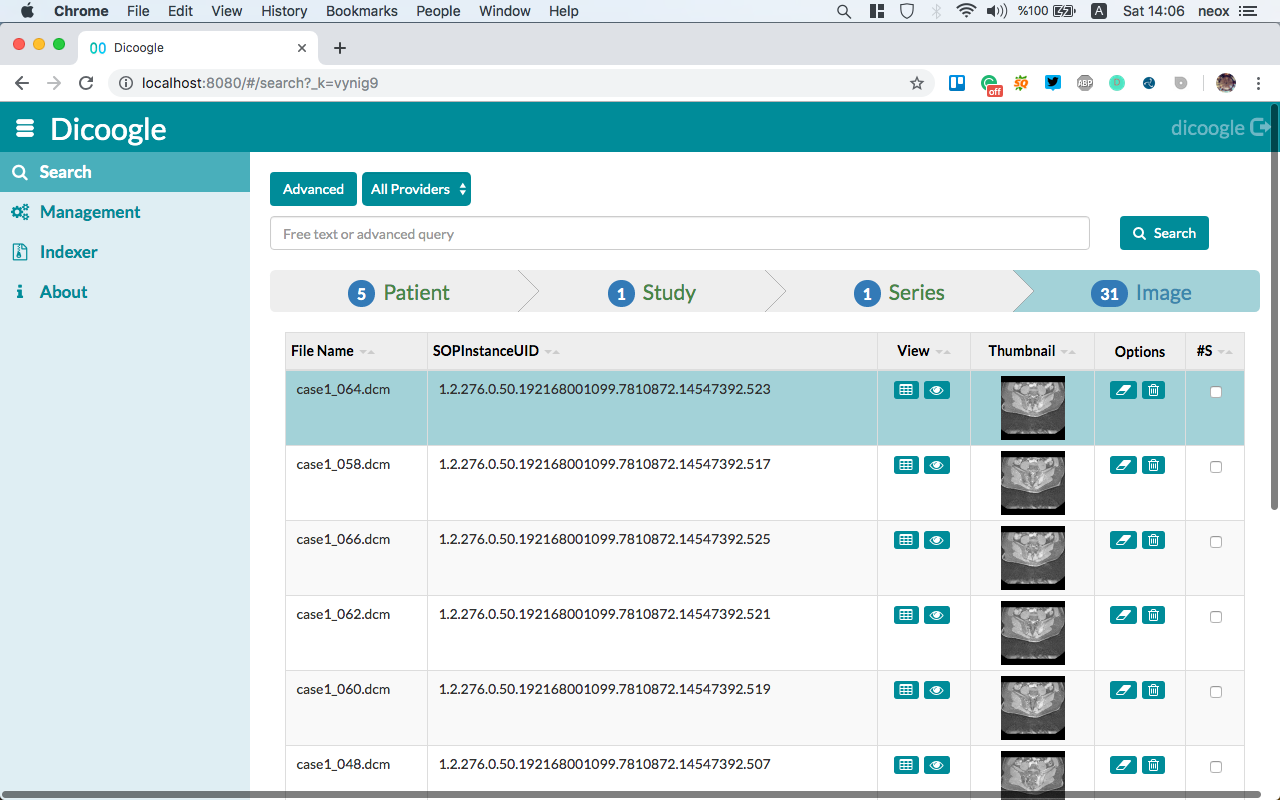
\includegraphics[width=0.4\textwidth]{dicoogle.png}
    \caption{Dicoogle界面}
    \label{fig:Dicoogle}
\end{figure}

\subsubsection{Orthanc}
Orthanc 是一个开源、模块化、轻量级的 DICOM 服务器项目,由比利时的列日大学医院与2012年9月发起。它配备了丰富的API 和几个插件,支持不同的数据库和DICOM查看者。Orthanc可在Linux、Windows等多平台下运行,执行GPL开源协议。

\begin{figure}[H]
    \centering
    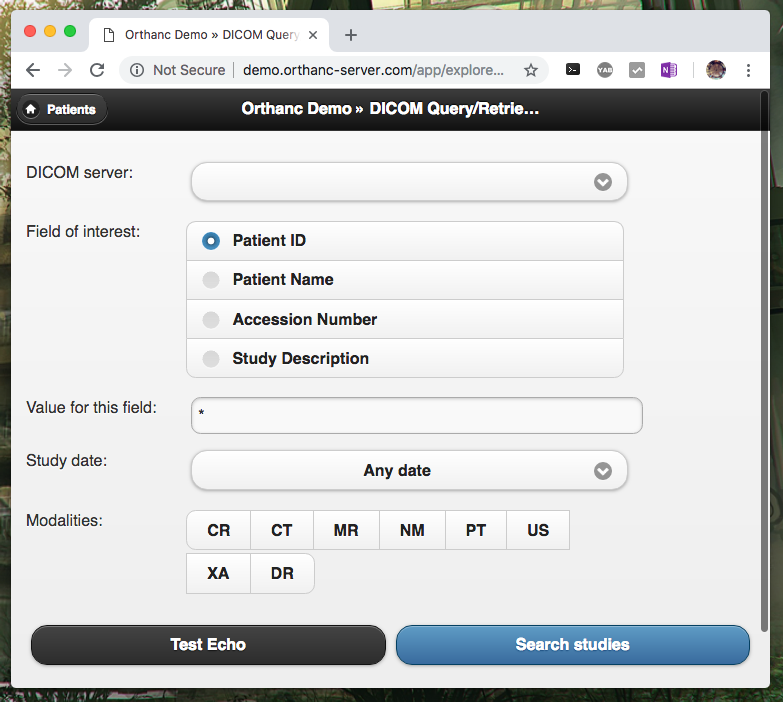
\includegraphics[width=0.4\textwidth]{orthanc.png}
    \caption{Orthanc界面}
    \label{fig:Orthanc}
\end{figure}


\subsection{开源医学图像处理软件}
\subsubsection{ITK}
ITK(Insight Segmentation and Registration Toolkit)是一个跨平台、开源的应用程序开发框架,广泛用于图像分割和图像配准程序的开发。ITK 是在NLM的资助下开发的。该工具包提供了两个、三个和更多维度的前沿分割和配准算法。ITK使用CMake构建环境来管理配置过程。该软件是用C++实现的,并为Python包装。SimpleITK是ITK项目的一个分支,以八种编程语言为ITK提供简化的接口,也在积极开发中。
\subsubsection{pydicom}
pydicom是一个使用纯Python语言的第三方库,它提供了在Python环境下读取、修改和写入Dicom文件的API。pydicom支持单张Dicom和序列的读取,并可以很容易的将Dicom像素数据转化为Numpy.ndarray格式,极大方便了医学图像处理工作者的进一步处理和可视化。同时pydicom也支持tag解析,和JPEG压缩方式的文件写入。

\subsection{生物信息学开源软件}
\subsubsection{EMBOSS}
EMBOSS(The European Molecular Biology Open Software Suite),是专为分子生物学研究用户的需要而开发的免费开源软件分析包。该软件自动处理各种格式的数据,甚至允许从 Web 上透明地检索序列数据。此外,由于提供了广泛的库,这是一个平台,让其他科学家开发和发布软件在真正的开源精神。EMBOSS 还将一系列当前可用的软件包和工具集成到整体中,以便进行序列分析。EMBOSS运行在Linux上,支持序列的信息提取、比对等各种常用功能,同时也提供了Web版。EMBOSS使用的是GPL和LGPL开源协议。
\subsubsection{Bioconductor}
Bioconductor是一款基于R语言开发的开源软件,可用于高通量的基因组数据。Bioconductor追求的是透明开源、可重复性和高效开发。R语言在统计中本来就占有压倒性的地位,R语言支持面向对象、互联网接口、并行计算、可视化、统计模拟和建模等各类适合处理高通量基因组处理的语言特性,这也为Bioconductor打下了基础,Bioconductor建议同时发表数据和每一步执行的命令,而不是只提供算法,这大大提高了可重复性实验的操作难度。此外,Bioconductor还支持动态的生物注释,可以随着研究的进行更新生物信息的注释。

\section{结果与讨论}


\bibliography{references}
\end{document}
